\chapter{Matrices, Linear Algebra and Linear Programming}\label{chap:Matrices}
In this section, we will review matrix concepts critical for the general understanding of general linear programming algorithms. 

Let $\mathbf{x}$ and $\mathbf{y}$ be two vectors in $\mathbb{R}^n$. Recall we denote the dot product of the two vectors as $\mathbf{x} \cdot \mathbf{y}$. 

\section{Matrices}
Recall an $m \times n$ matrix is a rectangular array of numbers, usually drawn from a field such as $\mathbb{R}$. We write an $m \times n$ matrix with values in $\mathbb{R}$ as $\mathbf{A} \in \mathbb{R}^{m \times n}$. The matrix consists of $m$ rows and $n$ columns. The element in the $i^\text{th}$ row and $j^\text{th}$ column of $\mathbf{A}$ is written as $\mathbf{A}_{ij}$. The $j^\text{th}$ column of $\mathbf{A}$ can be written as $\mathbf{A}_{\cdot j}$, where the $\cdot$ is interpreted as ranging over every value of $i$ (from $1$ to $m$). Similarly, the $i^{th}$ row of $\mathbf{A}$ can be written as $\mathbf{A}_{i\cdot}$. When $m = n$, then the matrix $\mathbf{A}$ is called \textit{square}.

\begin{definition}[Matrix Addition]
If $\mathbf{A}$ and $\mathbf{B}$ are both in $\mathbb{R}^{m \times n}$, then $\mathbf{C} = \mathbf{A} + \mathbf{B}$ is the matrix sum of $\mathbf{A}$ and $\mathbf{B}$ and 
\begin{equation}
\mathbf{C}_{ij} = \mathbf{A}_{ij} + \mathbf{B}_{ij}\;\; \text{for $i=1,\dots,m$ and $j=1,\dots,n$}
\end{equation}
\end{definition}

\begin{example} 
\begin{equation}
\left[
\begin{array}{cc}
1 & 2\\
3 & 4
\end{array}
\right] + 
\left[
\begin{array}{cc}
5 & 6\\
7 & 8
\end{array}
\right] = 
\left[
\begin{array}{cc}
1 + 5 & 2 + 6\\
3 + 7 & 4 + 8
\end{array}
\right] = 
\left[
\begin{array}{cc}
6 & 8\\
10 & 12
\end{array}
\right]
\end{equation}
\end{example}

\begin{definition}[Row/Column Vector]
A $1 \times n$ matrix is called a \textit{row vector}, and a $m \times 1$ matrix is called a \textit{column vector}. For the remainder of these notes, every vector will be thought of \textbf{column vector} unless otherwise noted.
\end{definition}

It should be clear that any row of matrix $\mathbf{A}$ could be considered a row vector in $\mathbb{R}^n$ and any column of $\mathbf{A}$ could be considered a column vector in $\mathbb{R}^m$.

\begin{definition}[Matrix Multiplication]
If $\mathbf{A} \in \mathbb{R}^{m \times n}$ and $B \in \mathbb{R}^{n \times p}$, then $\mathbf{C} = \mathbf{A}\mathbf{B}$ is the \textit{matrix product} of $\mathbf{A}$ and $\mathbf{B}$ and
\begin{equation}
\mathbf{C}_{ij} = \mathbf{A}_{i\cdot} \cdot \mathbf{B}_{\cdot j}
\end{equation}
Note, $\mathbf{A}_{i\cdot} \in \mathbb{R}^{1 \times n}$ (an $n$-dimensional vector) and $\mathbf{B}_{\cdot j} \in \mathbb{R}^{n \times 1}$ (another $n$-dimensional vector), thus making the dot product meaningful. 
\end{definition}

\begin{example} 
\begin{equation}
\left[
\begin{array}{cc}
1 & 2\\
3 & 4
\end{array}
\right] 
\left[
\begin{array}{cc}
5 & 6\\
7 & 8
\end{array}
\right] = 
\left[
\begin{array}{cc}
1(5) + 2(7) & 1(6) + 2(8)\\
3(5) + 4(7) & 3(6) + 4(8)
\end{array}
\right] = 
\left[
\begin{array}{cc}
19 & 22\\
43 & 50
\end{array}
\right]
\end{equation}
\end{example}

\begin{definition}[Matrix Transpose] If $\mathbf{A} \in \mathbb{R}^{m \times n}$ is a $m \times n$ matrix, then the \textit{transpose} of $\mathbf{A}$ dented $\mathbf{A}^T$ is an $m \times n$ matrix defined as:
\begin{equation}
\mathbf{A}^T_{ij} = \mathbf{A}_{ji}
\end{equation}
\end{definition}
\begin{example}
\begin{equation}
\left[
\begin{array}{cc}
1 & 2\\
3 & 4
\end{array}
\right]^T = 
\left[
\begin{array}{cc}
1 & 3\\
2 & 4
\end{array}
\right] 
\end{equation}
\end{example}

The matrix transpose is a particularly useful operation and makes it easy to transform column vectors into row vectors, which enables multiplication. For example, suppose $\mathbf{x}$ is an $n \times 1$ column vector (i.e., $\mathbf{x}$ is a vector in $\mathbb{R}^n$) and suppose $\mathbf{y}$ is an $n \times 1$ column vector. Then:
\begin{equation}
\mathbf{x} \cdot \mathbf{y} = \mathbf{x}^T\mathbf{y}
\end{equation}

\begin{exercise} Let $\mathbf{A}, \mathbf{B} \in \mathbb{R}^{m \times n}$. Use the definitions of matrix addition and transpose to prove that:
\begin{equation}
(\mathbf{A} + \mathbf{B})^T = \mathbf{A}^T + \mathbf{B}^T
\end{equation}
[Hint: If $\mathbf{C} = \mathbf{A} + \mathbf{B}$, then $\mathbf{C}_{ij} = \mathbf{A}_{ij} + \mathbf{B}_{ij}$, the element in the $(i,j)$ position of matrix $\mathbf{C}$. This element moves to the $(j,i)$ position in the transpose. The $(j,i)$ position of $\mathbf{A}^T + \mathbf{B}^T$ is $\mathbf{A}_{ji}^T + \mathbf{B}^T_{ji}$, but $\mathbf{A}_{ji}^T = \mathbf{A}_{ij}$. Reason from this point.] 
\label{exer:AdditionTranspose}
\end{exercise}

\begin{exercise} Let $\mathbf{A}, \mathbf{B} \in \mathbb{R}^{m \times n}$. Prove by example that $\mathbf{A}\mathbf{B} \neq \mathbf{B}\mathbf{A}$; that is, matrix multiplication is \textit{not commutative}. [Hint: Almost any pair of matrices you pick (that can be multiplied) will not commute.]
\end{exercise}

\begin{exercise} Let $\mathbf{A} \in \mathbb{R}^{m \times n}$ and let, $\mathbf{B} \in \mathbb{R}^{n \times p}$. Use the definitions of matrix multiplication and transpose to prove that:
\begin{equation}
(\mathbf{A}\mathbf{B})^T = \mathbf{B}^T\mathbf{A}^T
\end{equation}
[Hint: Use similar reasoning to the hint in Exercise \ref{exer:AdditionTranspose}. But this time, note that $\mathbf{C}_{ij} = \mathbf{A}_{i\cdot} \cdot \mathbf{B}_{\cdot j}$, which moves to the $(j,i)$ position. Now figure out what is in the $(j,i)$ position of $\mathbf{B}^T\mathbf{A}^T$.]
\end{exercise}

Let $\mathbf{A}$ and $\mathbf{B}$ be two matrices with the same number of rows (so $\mathbf{A} \in \mathbb{R}^{m \times n}$ and $\mathbf{B} \in \mathbb{R}^{m \times p}$). Then the augmented matrix $\left[\mathbf{A}|\mathbf{B}\right]$ is:
\begin{equation}
\left[
\begin{array}{cccc|cccc}
a_{11} & a_{12} & \dots & a_{1n} & b_{11} & b_{12} & \dots & b_{1p}\\
a_{21} & a_{22} & \dots & a_{2n} & b_{21} & b_{22} & \dots & b_{2p}\\
\vdots & & \ddots & \vdots & \vdots & & \ddots & \vdots\\
a_{m1} & a_{m2} & \dots & a_{mn} & b_{m1} & b_{m2} & \dots & b_{mp}\\
\end{array}
\right]
\end{equation}
Thus, $\left[\mathbf{A}|\mathbf{B}\right]$ is a matrix in $\mathbb{R}^{m \times (n + p)}$. 

\begin{example} Consider the following matrices:
\begin{displaymath}
\mathbf{A} = \left[ 
\begin{array}{cc}
1 & 2\\
3 & 4
\end{array}
\right],\;\;\;\mathbf{b} = \left[
\begin{array}{c}
7\\
8
\end{array}
\right]
\end{displaymath}
Then $\left[\mathbf{A}|\mathbf{B}\right]$ is:
\begin{displaymath}
\left[\mathbf{A}|\mathbf{B}\right] = \left[ 
\begin{array}{cc|c}
1 & 2 & 7\\
3 & 4 & 8
\end{array}
\right]
\end{displaymath}
\end{example}

\begin{exercise} By analogy define the augmented matrix $\left[\frac{\mathbf{A}}{\mathbf{B}}\right]$. Note, this is \textbf{not} a fraction. In your definition, identify the appropriate requirements on the relationship between the number of rows and columns that the matrices must have. [Hint: Unlike $\left[\mathbf{A}|\mathbf{B}\right]$, the number of rows don't have to be the same, since your concatenating on the rows, not columns. There should be a relation between the numbers of columns though.]
\end{exercise}

\section{Special Matrices and Vectors}
\begin{definition}[Identify Matrix] The $n \times n$ \textit{identify matrix} is:
\begin{equation}
\mathbf{I}_n = 
\left[
\begin{array}{cccc}
1 & 0 & \dots & 0\\
0 & 1 & \dots & 0\\
\vdots & & \ddots & \vdots\\
0 & 0 & \dots & 1
\end{array}\right]
\end{equation}
\end{definition}
When it is clear from context, we may simply write $\mathbf{I}$ and omit the subscript $n$. 
\begin{exercise} Let $\mathbf{A} \in \mathbb{R}^{n \times n}$. Show that $\mathbf{A}\mathbf{I}_n = \mathbf{I}_n\mathbf{A} = \mathbf{A}$. Hence, $\mathbf{I}$ is an identify for the matrix multiplication operation on square matrices. [Hint: Do the multiplication out long hand.]
\end{exercise}
\begin{definition}[Standard Basis Vector] The standard basis vector $\mathbf{e}_i \in \mathbb{R}^n$ is:
\begin{displaymath}
\mathbf{e}_i = \left(\underset{i-1}{\underbrace{0,0,\dots}},1,
\underset{n-i-1}{\underbrace{0,\dots,0}}\right)
\end{displaymath}
Note, this definition is only valid for $n \geq i$. Further the standard basis vector $\mathbf{e}_i$ is also the $i^{\text{th}}$ row or column of $\mathbf{I}_n$. 
\end{definition}

\begin{definition}[Unit and Zero Vectors] The vector $\mathbf{e} \in \mathbb{R}^n$ is the \textit{one vector} $\mathbf{e} = (1,1,\dots,1)$. Similarly, the \textit{zero vector} $\mathbf{0} = (0,0,\dots,0) \in \mathbb{R}^n$. We assume that the length of $\mathbf{e}$ and $\mathbf{0}$ will be determined from context. 
\end{definition}

\begin{exercise} Let $\mathbf{x} \in \mathbb{R}^n$, considered as a column vector (our standard assumption). Define:
\begin{displaymath}
\mathbf{y} = \frac{\mathbf{x}}{\mathbf{e}^T\mathbf{x}}
\end{displaymath}
Show that $\mathbf{e}^T\mathbf{y} = \mathbf{y}^T\mathbf{e} = 1$. [Hint: First remember that $\mathbf{e}^T\mathbf{x}$ is a scalar value (it's $\mathbf{e}\cdot\mathbf{x}$. Second, remember that a scalar times a vector is just a new vector with each term multiplied by the scalar. Last, use these two pieces of information to write the product $\mathbf{e}^T\mathbf{y}$ as a sum of fractions.]
\end{exercise}

\section{Matrices and Linear Programming Expression}
You will recall from your matrices class (Math 220) that matrices can be used as a short hand way to represent linear equations. Consider the following system of equations:
\begin{equation}
\left\{
\begin{aligned}
a_{11}x_1 + a_{12}x_2 + \dots + a_{1n}x_n & = b_1\\
a_{21}x_1 + a_{22}x_2 + \dots + a_{2n}x_n & = b_2\\
\vdots\\
a_{m1}x_1 + a_{m2}x_2 + \dots + a_{mn}x_n & = b_m
\end{aligned}\right.
\label{eqn:LinearEqns}
\end{equation}
Then we can write this in matrix notation as:
\begin{equation}
\mathbf{A}\mathbf{x} = \mathbf{b}
\end{equation}
where $\mathbf{A}_{ij} = a_{ij}$ for $i=1,\dots,m$, $j=1,\dots,n$ and $\mathbf{x}$ is a column vector in $\mathbb{R}^n$ with entries $x_j$ ($j=1,\dots,n$) and $\mathbf{b}$ is a column vector in $\mathbb{R}^m$ with entries $b_i$ ($i=1\dots,m$). Obviously, if we replace the equalities in Expression \ref{eqn:LinearEqns} with inequalities, we can also express systems of inequalities in the form:
\begin{equation}
\mathbf{A}\mathbf{x} \leq \mathbf{b}
\end{equation}

Using this representation, we can write our general linear programming problem using matrix and vector notation. Expression \ref{eqn:GeneralLPMax} can be written as:
\begin{equation}
\left\{
\begin{aligned}
\max\;\; z(\mathbf{x}) = &\mathbf{c}^T\mathbf{x}\\
s.t.\;\;&\mathbf{A}\mathbf{x} \leq \mathbf{b}\\
& \mathbf{H}\mathbf{x} = \mathbf{r}
\end{aligned}\right.
\label{eqn:GeneralLPMaxMatrixForm}
\end{equation}

For historical reasons, linear programs are not written in the general form of Expression \ref{eqn:GeneralLPMaxMatrixForm}. 

\begin{definition}[Canonical Form]  A maximization linear programming problem is in \textit{canonical form} if it is written as:
\begin{equation}
\left\{
\begin{aligned}
\max\;\; z(\mathbf{x}) = &\mathbf{c}^T\mathbf{x}\\
s.t.\;\;&\mathbf{A}\mathbf{x} \leq \mathbf{b}\\
& \mathbf{x} \geq \mathbf{0}
\end{aligned}\right.
\label{eqn:CanonicalFormMax}
\end{equation}

A minimization linear programming problem is in \textit{canonical form} if it is written as:
\begin{equation}
\left\{
\begin{aligned}
\min\;\; z(\mathbf{x}) = &\mathbf{c}^T\mathbf{x}\\
s.t.\;\;&\mathbf{A}\mathbf{x} \geq \mathbf{b}\\
& \mathbf{x} \geq \mathbf{0}
\end{aligned}\right.
\label{eqn:MinCanonicalFormMax}
\end{equation}
\end{definition}

\begin{definition}[Standard Form (Max Problem)]  A maximization linear programming problem is in \textit{standard form} if it is written as:
\begin{equation}
\left\{
\begin{aligned}
\max\;\; z(\mathbf{x}) = &\mathbf{c}^T\mathbf{x}\\
s.t.\;\;&\mathbf{A}\mathbf{x} = \mathbf{b}\\
& \mathbf{x} \geq \mathbf{0}
\end{aligned}\right.
\label{eqn:StandardFormMax}
\end{equation}
\end{definition}

\begin{remark} In the previous definition, a problem is in standard form as long as its constraints have form $\mathbf{A}\mathbf{x} = \mathbf{b}$ and $\mathbf{x} \geq \mathbf{0}$. The problem can be either a maximization or minimization problem.
\end{remark}


\begin{theorem}Every linear programming problem in canonical form can be put into standard form.
\end{theorem}
\begin{proof} Consider the constraint corresponding to the first row of the matrix $\mathbf{A}$:
\begin{equation}
a_{11}x_1 + a_{12}x_2 + \dots + a_{1n}x_n \leq b_1
\end{equation}
Then we can add a new \textit{slack} variable $s_1$ so that $s_1 \geq 0$ and we have:
\begin{equation}
a_{11}x_1 + a_{12}x_2 + \dots + a_{1n}x_n + s_1 = b_1
\end{equation}
This act can be repeated for each row of $\mathbf{A}$ (constraint) yielding $m$ new variables $s_1,\dots,s_m$, which we can express as a row $\mathbf{s}$. Then the new linear programming problem can be expressed as:
\begin{displaymath}
\left\{
\begin{aligned}
\max\;\; z(\mathbf{x}) = &\mathbf{c}^T\mathbf{x}\\
s.t.\;\;&\mathbf{A}\mathbf{x} + \mathbf{I}_m\mathbf{s}= \mathbf{b}\\
& \mathbf{x},\mathbf{s} \geq \mathbf{0}
\end{aligned}\right.
\label{eqn:CanonicalFormMax}
\end{displaymath}

Using augmented matrices, we can express this as:
\begin{displaymath}
\left\{
\begin{aligned}
\max\;\; z(\mathbf{x}) = &\left[\frac{\mathbf{c}}{\mathbf{0}}\right]^T\left[\frac{\mathbf{x}}{\mathbf{s}}\right]\\
s.t.\;\;&\left[\mathbf{A}|\mathbf{I}_m\right]\left[\frac{\mathbf{x}}{\mathbf{s}}\right]= \mathbf{b}\\
& \left[\frac{\mathbf{x}}{\mathbf{s}}\right] \geq \mathbf{0}
\end{aligned}\right.
\label{eqn:CanonicalFormMax}
\end{displaymath}
Clearly, this new linear programming problem is in standard form and any solution maximizing the original problem will necessarily maximize this one.
\end{proof}

\begin{example} Consider the Toy Maker problem from Example \ref{ex:ToyMaker}. The problem in canonical form is:
\begin{displaymath}
\left\{
\begin{aligned}
\max\;\;& z(x_1,x_2) = 7x_1 + 6x_2\\
s.t.\;\;&  3x_1 + x_2 \leq 120\\
& x_1 + 2x_2 \leq 160\\
& x_1 \leq 35\\
& x_1 \geq 0\\
& x_2 \geq 0
\end{aligned}
\right.
\end{displaymath}
We can introduce slack variables $s_1$, $s_2$ and $s_3$ into the constraints (one for each constraint) and re-write the problem as:
\begin{displaymath}
\left\{
\begin{aligned}
\max\;\;& z(x_1,x_2) = 7x_1 + 6x_2\\
s.t.\;\;&  3x_1 + x_2 + s_1 = 120\\
& x_1 + 2x_2 + s_2 = 160\\
& x_1 + s_3 = 35\\
& x_1 \geq 0\\
& x_2 \geq 0
\end{aligned}
\right.
\end{displaymath}
\label{ex:ToyMakerStandard}
\end{example}

\begin{remark}
We can deal with constraints of the form:
\begin{equation}
a_{i1}x_1 + a_{i2}x_2 + \dots + a_{in}x_n \geq b_i
\label{eqn:GTConstraint}
\end{equation}
in a similar way. In this case we subtract a surplus variable $s_i$ to obtain:
\begin{displaymath}
a_{i1}x_1 + a_{i2}x_2 + \dots + a_{in}x_n - s_i = b_i
\end{displaymath}
Again, we must have $s_i \geq 0$. 
\end{remark}

\begin{theorem} Every linear programming problem in standard form can be put into canonical form.
\end{theorem}
\begin{proof} Recall that $\mathbf{A}\mathbf{x} = \mathbf{b}$ if and only if $\mathbf{A}\mathbf{x} \leq \mathbf{b}$ and $\mathbf{A}\mathbf{x} \geq \mathbf{b}$. The second inequality can be written as $-\mathbf{A}\mathbf{x} \leq -\mathbf{b}$. This yields the linear programming problem:
\begin{equation}
\left\{
\begin{aligned}
\max\;\; z(\mathbf{x}) = &\mathbf{c}^T\mathbf{x}\\
s.t.\;\;&\mathbf{A}\mathbf{x} \leq \mathbf{b}\\
& -\mathbf{A}\mathbf{x} \leq -\mathbf{b}\\
& \mathbf{x} \geq \mathbf{0}
\end{aligned}\right.
\label{eqn:StandardConversion}
\end{equation}
Defining the appropriate augmented matrices allows us to convert this linear programming problem into canonical form.
\end{proof}
\begin{exercise} Complete the ``pedantic'' proof of the preceding theorem by defining the correct augmented matrices to show that the linear program in Expression \ref{eqn:StandardConversion} is in canonical form.
\end{exercise}

The standard solution method for linear programming models (the Simplex Algorithm) assumes that all variables are non-negative. Though this assumption can be easily relaxed, the first implementation we will study imposes this restriction. The general linear programming problem we posed in Expression \ref{eqn:GeneralLPMaxMatrixForm} does not (necessarily) impose any sign restriction on the variables. We will show that we can transform a problem in which $x_i$ is unrestricted into a new problem in which all variables are positive. Clearly, if $x_i \leq 0$, then we simply replace $x_i$ by $-y_i$ in every expression and then $y_i \geq 0$. On the other hand, if we have the constraint $x_i \geq l_i$, then clearly we can write $y_i = x_i - l_i$ and $y_i \geq 0$. We can then replace $x_i$ by $y_i + l_i$ in every equation or inequality where $x_i$ appears. Finally, if $x_i \leq u_i$, but $x_i$ may be negative, then we may write $y_i = u_i - x_i$. Clearly, $y_i \geq 0$ and we can replace $x_i$ by $u_i - y_i$ in every equation or inequality where $x_i$ appears. 

If $x_i$ is unrestricted in sign and has no upper or lower bounds, then let $x_i = y_i - z_i$ where $y_i, z_i \geq 0$ and replace $x_i$ by $(y_i-z_i)$ in the objective, equations and inequalities of a general linear programming problem. Since $y_i, z_i \geq 0$ and may be given any values as a part of the solution, clearly $x_i$ may take any value in $\mathbb{R}$. 
\begin{exercise} Convince yourself that the general linear programming problem shown in Expression \ref{eqn:GeneralLPMaxMatrixForm} can be converted into canonical (or standard) form using the following steps:
\begin{enumerate*}
\item Every constraint of the form $x_i \leq u_i$ can be dealt with by substituting $y_i = u_i - x_i$, $y_i \geq 0$.
\item Every constraint of the form $l_i \leq x_i$ can be dealt with by substituting $y_i = x_i - l_i$, $y_i \geq 0$.
\item If $x_i$ is unrestricted in any way, then we can variables $y_i$ and $z_i$ so that $x_i = y_i - z_i$ where $y_i, z_i \geq 0$.
\item Any equality constraints $\mathbf{H}\mathbf{x} = \mathbf{r}$ can be transformed into inequality constraints.
\end{enumerate*}
Thus, Expression \ref{eqn:GeneralLPMaxMatrixForm} can be transformed to standard form. [Hint: No hint, the hint is in the problem.]
\end{exercise}

\section{Gauss-Jordan Elimination and Solution to Linear Equations}
In this sub-section, we'll review Gauss-Jordan Elimination as a solution method for linear equations. We'll use Gauss-Jordan Elimination \textit{extensively} in the coming chapters. 

\begin{definition}[Elementary Row Operation] Let $\mathbf{A} \in \mathbb{R}^{m \times n}$ be a matrix. Recall $\mathbf{A}_{i \cdot}$ is the $i^\text{th}$ row of $\mathbf{A}$. There are three \textit{elementary row operations}:
\begin{enumerate}
\item (Scalar Multiplication of a Row) Row $\mathbf{A}_{i \cdot}$ is replaced by $\alpha \mathbf{A}_{i \cdot}$, where $\alpha \in \mathbb{R}$ and $\alpha \neq 0$. 
\item (Row Swap) Row $\mathbf{A}_{i \cdot}$ is swapped with Row $\mathbf{A}_{j \cdot}$ for $i \neq j$.
\item (Scalar Multiplication and Addition) Row $\mathbf{A}_{j \cdot}$ is replaced by $\alpha \mathbf{A}_{i \cdot} + \mathbf{A}_{j \cdot}$ for $\alpha \in \mathbb{R}$ and $i \neq j$.
\end{enumerate}
\end{definition}

\begin{example} Consider the matrix:
\begin{displaymath}
\mathbf{A} = 
\begin{bmatrix}
1 & 2\\
3 & 4
\end{bmatrix}
\end{displaymath}
In an example of scalar multiplication of a row by a constant, we can multiply the second row by $1/3$ to obtain:
\begin{displaymath}
\mathbf{B} = 
\begin{bmatrix}
1 & 2\\
1 & \frac{4}{3}
\end{bmatrix}
\end{displaymath}
As an example of scalar multiplication and addition, we can multiply the second row by $(-1)$ and add the result to the first row to obtain:
\begin{displaymath}
\mathbf{C} = 
\begin{bmatrix}
0 & 2-\frac{4}{3}\\
1 & \frac{4}{3}
\end{bmatrix} = 
\begin{bmatrix}
0 & \frac{2}{3}\\
1 & \frac{4}{3}
\end{bmatrix}
\end{displaymath}
We can then use scalar multiplication and multiply the first row by $(3/2)$ to obtain:
\begin{displaymath}
\mathbf{D} = 
\begin{bmatrix}
0 & 1\\
1 & \frac{4}{3}
\end{bmatrix}
\end{displaymath}

We can then use scalar multiplication and addition to multiply the first row by $(-4/3)$ add it to the second row to obtain:
\begin{displaymath}
\mathbf{E} = 
\begin{bmatrix}
0 & 1\\
1 & 0
\end{bmatrix}
\end{displaymath}
Finally, we can swap row 2 and row 1 to obtain:
\begin{displaymath}
\mathbf{I}_2 = 
\begin{bmatrix}
1 & 0\\
0 & 1
\end{bmatrix}
\end{displaymath}
Thus using elementary row operations, we have transformed the matrix $\mathbf{A}$ into the matrix $\mathbf{I}_2$.
\label{ex:ElemRowOps}
\end{example}

\begin{theorem} Each elementary row operation can be accomplished by a matrix multiplication.
\label{thm:ElemRowOpsAsMatrixMult}
\end{theorem}
\begin{proof} We'll show that scalar multiplication and row addition can be accomplished by a matrix multiplication. In Exercise \ref{exer:ElemRowOpsAsMatrixMult}, you'll be asked to complete the proof for the other two elementary row operations.

Let $\mathbf{A} \in \mathbb{R}^{m \times n}$. Without loss of generality, suppose we wish to multiply row $1$ by $\alpha$ and add it to row $2$, replacing row $2$ with the result. Let:
\begin{equation}
\mathbf{E} = \begin{bmatrix}
1 & 0 & 0 & \dots & 0\\
\alpha & 1 & 0 & \dots & 0\\
\vdots & \vdots & & \ddots & 0\\
0 & 0 & 0 & \dots & 1
\end{bmatrix}
\end{equation}
This is simply the identity $I_m$ with an $\alpha$ in the $(2,1)$ position instead of $0$. Now consider $\mathbf{E}\mathbf{A}$. Let $\mathbf{A}_{\cdot j} = [a_{1j},a_{2j},\dots,a_{mj}]^T$ be the $j^\text{th}$ column of $\mathbf{A}$. Then :
\begin{equation}
\begin{bmatrix}
1 & 0 & 0 & \dots & 0\\
\alpha & 1 & 0 & \dots & 0\\
\vdots & \vdots & & \ddots & 0\\
0 & 0 & 0 & \dots & 1
\end{bmatrix}
\begin{bmatrix}
a_{1j}\\
a_{2j}\\
\vdots\\
a_{mj}
\end{bmatrix} = 
\begin{bmatrix}
a_{1j}\\
\alpha(a_{1j}) + a_{2j}\\
\vdots\\
a_{mj}
\end{bmatrix}
\end{equation}
That is, we have taken the first element of $\mathbf{A}_{\cdot j}$ and multiplied it by $\alpha$ and added it to the second element of $\mathbf{A}_{\cdot j}$ to obtain the new second element of the product. All other elements of $\mathbf{A}_{\cdot j}$ are unchanged. Since we chose an arbitrary column of $\mathbf{A}$, it's clear this will occur in each case. Thus $\mathbf{E} \mathbf{A}$ will be the new matrix with rows the same as $\mathbf{A}$ \textit{except} for the second row, which will be replaced by the first row of $\mathbf{A}$ multiplied by the constant $\alpha$ and added to the second row of $\mathbf{A}$. To multiply the $i^\text{th}$ row of $\mathbf{A}$ and add it to the $j^\text{th}$ row, we would simply make a matrix $E$ by starting with $\mathbf{I}_m$ and replacing the $i^\text{th}$ element of row $j$ with $\alpha$.  
\end{proof}
\begin{exercise} Complete the proof by showing that scalar multiplication and row swapping can be accomplished by a matrix multiplication. [Hint: Scalar multiplication should be easy, given the proof above. For row swap, try multiplying matrix $\mathbf{A}$ from Example \ref{ex:ElemRowOps} by:
\begin{displaymath}
\begin{bmatrix}
0 & 1\\
1 & 0
\end{bmatrix}
\end{displaymath}
and see what comes out. Can you generalize this idea for arbitrary row swaps?]
\label{exer:ElemRowOpsAsMatrixMult}
\end{exercise}

Matrices of the kind we've just discussed are called \textit{elementary matrices}. Theorem \ref{thm:ElemRowOpsAsMatrixMult} will be important when we study efficient methods for solving linear programming problems. It tells us that \textit{any} set of elementary row operations can be performed by finding the right matrix. That is, suppose I list 4 elementary row operations to perform on matrix $A$. These elementary row operations correspond to for matrices $\mathbf{E}_1, \dots, \mathbf{E}_4$. Thus the transformation of $\mathbf{A}$ under these row operations can be written using only matrix multiplication as $\mathbf{B} = \mathbf{E}_4\cdots\mathbf{E}_1\mathbf{A}$. This representation is \textit{much} simpler for a computer to keep track of in algorithms that require the transformation of matrices by elementary row operations.

\begin{definition}[Row Equivalence] Let $\mathbf{A} \in \mathbb{R}^{m \times n}$ and let $\mathbf{B} \in \mathbb{R}^{m \times n}$. If there is a sequence of elementary matrices $\mathbf{E}_1,\dots,\mathbf{E}_k$ so that:
\begin{displaymath}
\mathbf{B} = \mathbf{E}_k\cdots\mathbf{E}_1\mathbf{A}
\end{displaymath}
then $\mathbf{A}$ and $\mathbf{B}$ are said to be \textit{row equivalent}.
\end{definition}


\section{Matrix Inverse}
\begin{definition}[Invertible Matrix] Let $\mathbf{A} \in \mathbb{R}^{n \times n}$ be a square matrix. If there is a matrix $\mathbf{A}^{-1}$ such that
\begin{equation}
\mathbf{A} \mathbf{A}^{-1} = \mathbf{A}^{-1} \mathbf{A} = \mathbf{I}_n
\end{equation}
then matrix $\mathbf{A}$ is said to be \textit{invertible} (or \textit{nonsingular}) and $\mathbf{A}^{-1}$ is called its \textit{inverse}. If \textbf{A} is not invertible, it is called a \textit{singular} matrix.
\end{definition}

\begin{exercise} Find the equivalent elementary row operation matrices for Example \ref{ex:ElemRowOps}. There should be five matrices $\mathbf{E}_1, \dots, \mathbf{E}_5$ corresponding to the five steps shown. Show that the product of these matrices (in the correct order) yields the identity matrix. Now compute the product $\mathbf{B} = \mathbf{E}_5\cdots\mathbf{E}_1$. Show that $\mathbf{B} = \mathbf{A}^{-1}$ [Hint: You've done most of the work.]
\label{exer:MatrixInv1}
\end{exercise}

The proof of the following theorem is beyond the scope of this class. Proofs can be found in \cite{Str87} (Chapter 2) and \cite{Cull72} (Chapter 1) and should be covered in a Linear Algebra course (Math 436). 
\begin{theorem} If $\mathbf{A} \in \mathbb{R}^{n \times n}$ is a square matrix and $\mathbf{X} \in \mathbb{R}^{n \times n}$ so that $\mathbf{X}\mathbf{A} = \mathbf{I}_n$, then:
\begin{enumerate}
\item $\mathbf{A}\mathbf{X} = \mathbf{I}_n$
\item $\mathbf{X} = \mathbf{A}^{-1}$
\item $\mathbf{A}$ and $\mathbf{A}^{-1}$ can be written as a product of elementary matrices.
\end{enumerate}
\end{theorem}

The process we've illustrated in Example \ref{ex:ElemRowOps} is an instance of Gauss-Jordan elimination and can be used to find the inverse of any matrix (or to solve systems of linear equations). This process is summarized in Algorithm \ref{alg:GaussJordanEliminationInv}. 
\begin{definition}[Pivoting]
In Algorithm \ref{alg:GaussJordanEliminationInv} when $\mathbf{A}_{ii} \neq 0$, the process performed in Steps 4 and 5 is called \textit{pivoting} on element $(i,i)$.
\end{definition}
We illustrate this algorithm in the following example.

\begin{algorithm}
\caption{Gauss-Jordan Elimination for Matrix Inversion}
\label{alg:GaussJordanEliminationInv}
\begin{center}
\begin{minipage}[t]{\textwidth-1em}
\underline{\textbf{Gauss-Jordan Elimination}}\\
\textit{Computing an Inverse}
\begin{enumerate*}
\item Let $\mathbf{A} \in \mathbb{R}^{n \times n}$. Let $\mathbf{X} = [\mathbf{A} | \mathbf{I}_n]$.
\item Let $i := 1$
\item If $\mathbf{X}_{ii} = 0$, then use row-swapping on $\mathbf{X}$ to replace row $i$ with a row $j$ ($j > i$) so that $\mathbf{X}_{ii} \neq 0$. If this is not possible, then $\mathbf{A}$ is not invertible.
\item Replace $\mathbf{X}_{i\cdot}$ by $(1/\mathbf{X}_{ii})\mathbf{X}_{i\cdot}$. Element $(i,i)$ of $\mathbf{X}$ should now be $1$.
\item For each $j \neq i$, replace $\mathbf{X}_{j\cdot}$ by $\frac{-\mathbf{X}_{ji}}{\mathbf{X}_{ii}}\mathbf{X}_{i\cdot} + \mathbf{X}_{j\cdot}$.
\item Set $i := i + 1$.
\item If $i > n$, then $\mathbf{A}$ has been replaced by $\mathbf{I}_n$ and $\mathbf{I}_n$ has been replaced by $\mathbf{A}^{-1}$ in $\mathbf{X}$. If $i \leq n$, then goto Line 3.
\end{enumerate*}
\end{minipage}
\end{center}
\end{algorithm}

\begin{example}
Again consider the matrix $\mathbf{A}$ from Example \ref{ex:ElemRowOps}. We can follow the steps in Algorithm \ref{alg:GaussJordanEliminationInv} to compute $\mathbf{A}^{-1}$. 
\begin{description}
\item[Step 1]
\begin{displaymath}
\mathbf{X} := \left[\begin{array}{cc|cc}
1 & 2 & 1 & 0\\
3 & 4 & 0 & 1
\end{array}\right]
\end{displaymath}

\item[Step 2] $i:=1$

\item[Step 3 and 4 ($i=1$)]
$\mathbf{A}_{11} = 1$, so no swapping is required. Furthermore, replacing 
$\mathbf{X}_{1\cdot}$ by $(1/1)\mathbf{X}_{1\cdot}$ will not change $\mathbf{X}$. 

\item[Step 5 ($i=1$)] We multiply row $1$ of $\mathbf{X}$ by $-3$ and add the result to row 2 of $\mathbf{X}$ to obtain:
\begin{displaymath}
\mathbf{X} := \left[\begin{array}{cc|cc}
1 & 2 & 1 & 0\\
0 & -2 & -3 & 1
\end{array}\right]
\end{displaymath}

\item[Step 6] $i:=1+1=2$ and $i = n$ so we return to Step 3.

\item[Steps 3 ($i=2$)] The new element $\mathbf{A}_{22} = -2 \neq 0$. Therefore, no swapping is required.

\item[Step 4 ($i=2$)]
We replace row 2 of $\mathbf{X}$ with row 2 of $\mathbf{X}$ multiplied by $-1/2$.
\begin{displaymath}
\mathbf{X} := \left[\begin{array}{cc|cc}
1 & 2 & 1 & 0\\
0 & 1 & \frac{3}{2} & -\frac{1}{2}
\end{array}\right]
\end{displaymath}

\item[Step 5 ($i=2$)] We multiply row $2$ of $\mathbf{X}$ by $-2$ and add the result to row 1 of $\mathbf{X}$ to obtain:
\begin{displaymath}
\mathbf{X} := \left[\begin{array}{cc|cc}
1 & 0 & -2 & 1\\
0 & 1 & \frac{3}{2} & -\frac{1}{2}
\end{array}\right]
\end{displaymath}

\item[Step 6 ($i=2$)] $i := 2 + 1 = 3$. We now have $i > n$ and the algorithm terminates.
\end{description}

Thus using Algorithm \ref{alg:GaussJordanEliminationInv} we have computed:
\begin{displaymath}
\mathbf{A}^{-1} = \left[\begin{array}{cc}
-2 & 1\\
\frac{3}{2} & -\frac{1}{2}
\end{array}\right]
\end{displaymath}
This value should be the result you obtained in Exercise \ref{exer:MatrixInv1}.
\label{ex:GaussJordanEliminationInv}
\end{example}

\begin{exercise} Does the matrix:
\begin{displaymath}
\mathbf{A} = \begin{bmatrix}
1 & 2 & 3\\
4 & 5 & 6\\
7 & 8 & 9
\end{bmatrix}
\end{displaymath}
have an inverse? [Hint: Use Gauss-Jordan elimination to find the answer.]
\end{exercise}

\begin{exercise}[\textbf{Bonus}] Implement Gauss-Jordan elimination in the programming language of your choice. Illustrate your implementation by using it to solve the previous exercise. [Hint: Implement sub-routines for each matrix operation. You don't have to write them as matrix multiplication, though in Matlab, it might speed up your execution. Then use these subroutines to implement each step of the Gauss-Jordan elimination.]
\end{exercise}

\section{Solution of Linear Equations}
Let $\mathbf{A} \in \mathbb{R}^{n \times n}$, $\mathbf{b} \in \mathbb{R}^n$. Consider the problem:
\begin{equation}
\mathbf{A}\mathbf{x} = \mathbf{b}
\label{eqn:LinEqn}
\end{equation}
There are three possible scenarios:
\begin{enumerate*}
\item There is a unique solution $\mathbf{x} = \mathbf{A}^{-1}\mathbf{b}$.
\item There are no solutions; i.e., there is no vector $\mathbf{x}$ so that $\mathbf{A}\mathbf{x} = \mathbf{b}$.
\item There are infinitely many solutions; i.e., there is an infinite set $\mathcal{X} \subseteq \mathbb{R}^n$ such that for all $\mathbf{x} \in \mathcal{X}$, $\mathbf{A}\mathbf{x} = \mathbf{b}$.
\end{enumerate*}

We can use Gauss-Jordan elimination to find a solution $\mathbf{x}$ to Equation \ref{eqn:LinEqn} when it occurs. Instead of operating on the augmented $\mathbf{X} = [\mathbf{A}|\mathbf{I}_n]$ in Algorithm \ref{alg:GaussJordanEliminationInv}, we use the augmented matrix $\mathbf{X} := [\mathbf{A}|\mathbf{b}]$. If the algorithm terminates with $\mathbf{A}$ replaced by $\mathbf{I}_n$, then the solution vector resides where $\mathbf{b}$ began. That is, $\mathbf{X}$ is transformed to $\mathbf{X} := [\mathbf{I}_n | \mathbf{A}^{-1}\mathbf{b}]$.

If the algorithm \textit{does not} terminate with $\mathbf{X} := [\mathbf{I}_n | \mathbf{A}^{-1}\mathbf{b}]$, then suppose the algorithm terminates with $\mathbf{X} := [\mathbf{A}' | \mathbf{b}']$. There is \textit{at least} one row in $\mathbf{A}'$ with all zeros. That is $\mathbf{A}'$ has the form:
\begin{equation}
\mathbf{A}'=\begin{bmatrix}
1 & 0 & \dots & 0\\
0 & 1 & \dots & 0\\
\vdots & & \ddots & \vdots\\

0 & 0 & \dots & 0\\
\vdots & & \ddots & \vdots\\
0 & 0 & \dots & 0
\end{bmatrix}
\end{equation}
In this case, there are two possibilities:
\begin{enumerate*}
\item For every zero row in $\mathbf{A}'$, the corresponding element in $\mathbf{b'}$ is 0. In this case, there are an infinite number of alternative solutions to the problem expressed by Equation \ref{eqn:LinEqn}. 
\item There is at least one zero row in $\mathbf{A}'$ whose corresponding element in $\mathbf{b}'$ is not zero. In this case, there are no solutions to Equation \ref{eqn:LinEqn}.
\end{enumerate*}

We illustrate these two possibilities in the following example:
\begin{example}
Consider the system of equations:
\begin{displaymath}
\begin{aligned}
x_1 + 2x_2 + 3x_3 & = 7\\
4x_1 + 5x_2 + 6x_3 & = 8\\
7x_1 + 8x_2 + 9x_3 & =9
\end{aligned}
\end{displaymath}
This yields matrix:
\begin{displaymath}
\mathbf{A} = \begin{bmatrix}
1 & 2 & 3\\
4 & 5 & 6\\
7 & 8 & 9
\end{bmatrix}
\end{displaymath} 
and right hand side vector $\mathbf{b} = [7, 8, 9]^T$. Applying Gauss-Jordan elimination in this case yields:
\begin{equation}
\mathbf{X} :=
\left[
\begin{array}{ccc|c}
1 & 0 & -1 & -\frac{19}{3}\\
0 & 1 & 2 & \frac{20}{3}\\
0 & 0 & 0 & 0
\end{array}
\right]
\label{eqn:RowEchelon}
\end{equation}
Since the third row is all zeros, there are an infinite number of solutions. An easy way to solve for this set of equations is to let $x_3 = t$, where $t$ may take on any value in $\mathbb{R}$. Then, row 2 of Expression \ref{eqn:RowEchelon} tells us that:
\begin{equation}
x_2 + 2x_3 = \frac{20}{3} \implies x_2 + 2t = \frac{20}{3} \implies 
x_2 = \frac{20}{3} - 2t
\end{equation}
We then solve for $x_1$ in terms of $t$. From row 1 of Expression \ref{eqn:RowEchelon} we have:
\begin{equation}
x_1 - x_3 = -\frac{19}{3} \implies x_1 - t = -\frac{19}{3} \implies 
x_1 = t-\frac{19}{3}
\end{equation}

Thus every vector in the set:
\begin{equation}
\mathcal{X} = \left\{\left(t-\frac{19}{3}, \frac{20}{3} - 2t, t\right) : t \in \mathbb{R}\right\}
\end{equation}
is a solution to $\mathbf{A}\mathbf{x} = \mathbf{b}$. 

Conversely, suppose we have the problem:
\begin{displaymath}
\begin{aligned}
x_1 + 2x_2 + 3x_3 & = 7\\
4x_1 + 5x_2 + 6x_3 & = 8\\
7x_1 + 8x_2 + 9x_3 & =10
\end{aligned}
\end{displaymath}
The new right hand side vector is $\mathbf{b} = [7, 8, 20]^T$. Applying Gauss-Jordan elimination in this case yields:
\begin{equation}
\mathbf{X} :=
\left[
\begin{array}{ccc|c}
1 & 0 & -1 & 0\\
0 & 1 & 2 & 0\\
0 & 0 & 0 & 1
\end{array}
\right]
\label{eqn:RowEchelon2}
\end{equation}
Since row 3 of $\mathbf{X}$ has a non-zero element in the $\mathbf{b}'$ column, we know this problem has no solution, since there is no way that we can find values for $x_1$, $x_2$ and $x_3$ satisfying:
\begin{equation}
0x_1 + 0x_2 + 0x_3 = 1
\end{equation}
\end{example}

\begin{exercise}
Solve the problem
\begin{displaymath}
\begin{aligned}
x_1 + 2x_2 & = 7\\
3x_1 + 4x_2 & = 8
\end{aligned}
\end{displaymath}
using Gauss-Jordan elimination.
\end{exercise}

\section{Linear Combinations, Span, Linear Independence}
\begin{definition} Let $\mathbf{x}_1,\dots,\mathbf{x}_m$ be vectors in $\in \mathbb{R}^n$ and let $\alpha_1,\dots,\alpha_m \in \mathbb{R}$ be scalars. Then 
\begin{equation}
\alpha_1\mathbf{x}_1 + \dots + \alpha_m\mathbf{x}_m
\end{equation}
is a \textit{linear combination} of the vectors $\mathbf{x}_1,\dots,\mathbf{x}_m$.
\end{definition}

Clearly, any linear combination of vectors in $\mathbb{R}^n$ is also a vector in $\mathbb{R}^n$.

\begin{definition}[Span] Let $\mathcal{X} = \{\mathbf{x}_1,\dots,\mathbf{x}_m\}$ be a set of vectors in $\in \mathbb{R}^n$, then the span of $\mathcal{X}$ is the set:
\begin{equation}
\mathrm{span}(\mathcal{X}) = \left\{\mathbf{y} \in \mathbb{R}^n | \text{$\mathbf{y}$ is a linear combination of vectors in $\mathcal{X}$}\right\}
\end{equation}
\end{definition}

\begin{definition}[Linear Independence] Let $\mathbf{x}_1,\dots,\mathbf{x}_m$ be vectors in $\in \mathbb{R}^n$. The vectors $\mathbf{x}_1,\dots,\mathbf{x}_m$ are \textit{linearly dependent} if there exists $\alpha_1,\dots,\alpha_m \in \mathbb{R}$, not all zero, such that 
\begin{equation}
\alpha_1\mathbf{x}_1 + \dots + \alpha_m\mathbf{x}_m = \mathbf{0} 
\label{eqn:LinIndep}
\end{equation}
If the set of vectors $\mathbf{x}_1,\dots,\mathbf{x}_m$ is not linearly dependent, then they are \textit{linearly independent} and Equation \ref{eqn:LinIndep} holds just in case $\alpha_i = 0$ for all $i=1,\dots,n$. 
\end{definition}

\begin{exercise} Consider the vectors $\mathbf{x}_1 = [0,0]^T$ and $\mathbf{x}_2 = [1,0]^T$. Are these vectors linearly independent? Explain why or why not.
\end{exercise}

\begin{example} In $\mathbb{R}^3$, consider the vectors:
\begin{displaymath}
\mathbf{x}_1 = \begin{bmatrix}
1\\1\\0
\end{bmatrix},\;
\mathbf{x}_2 = \begin{bmatrix}
1\\0\\1
\end{bmatrix},\;
\mathbf{x}_3 = \begin{bmatrix}
0\\1\\1
\end{bmatrix}
\end{displaymath}
We can show these vectors are linearly independent: Suppose there are values $\alpha_1, \alpha_2, \alpha_3\in \mathbb{R}$ such that 
\begin{displaymath}
\alpha_1\mathbf{x}_1 + \alpha_2\mathbf{x}_2 + \alpha_3\mathbf{x}_3 = 0
\end{displaymath}
Then:
\begin{displaymath}
\begin{bmatrix}
\alpha_1\\\alpha_1\\0 
\end{bmatrix} + 
\begin{bmatrix}
\alpha_2\\0\\ \alpha_2
\end{bmatrix}
\begin{bmatrix}
0\\\alpha_3\\ \alpha_3
\end{bmatrix} = 
\begin{bmatrix}
\alpha_1+\alpha_2\\
\alpha_1 + \alpha_3 \\
\alpha_2 + \alpha_3
\end{bmatrix}=
\begin{bmatrix}
0\\0\\0
\end{bmatrix}
\end{displaymath}
Thus we have the system of linear equations:
\begin{displaymath}
\begin{aligned}
&\alpha_1  &+\alpha_2 &&= 0\\
&\alpha_1   &&+\alpha_3 &= 0 \\
&&\alpha_2  &+\alpha_3  &= 0
\end{aligned}
\end{displaymath}
which can be written as the matrix expression:
\begin{displaymath}
\begin{bmatrix}
1 & 1 & 0\\
1 & 0 & 1\\
0 & 1 & 1
\end{bmatrix}
\begin{bmatrix}
\alpha_1\\
\alpha_2\\
\alpha_3
\end{bmatrix}=
\begin{bmatrix}
0\\
0\\
0
\end{bmatrix}
\end{displaymath}
This is just a simple matrix equation, but note that the three vectors we are focused on: $\mathbf{x}_1$, $\mathbf{x}_2$, and $\mathbf{x}_3$, have become the \textit{columns} of the matrix on the left-hand-side. We can use Gauss-Jordan elimination to solve this matrix equation yielding: $\alpha_1 = \alpha_2 = \alpha_3 = 0$. Thus these vectors are linearly independent.
\label{ex:LinIndep1}
\end{example}

\begin{remark} It is worthwhile to note that the zero vector $\mathbf{0}$ makes any set of vectors a linearly dependent set.
\end{remark}

\begin{exercise} Prove the remark above.
\end{exercise}

\begin{exercise} Show that the vectors 
\begin{displaymath}
\mathbf{x}_1 = \begin{bmatrix}
1\\2\\3
\end{bmatrix},\;
\mathbf{x}_2 = \begin{bmatrix}
4\\5\\6
\end{bmatrix},\;
\mathbf{x}_3 = \begin{bmatrix}
7\\8\\9
\end{bmatrix}
\end{displaymath}
are \textit{not} linearly independent. [Hint: Following the example, create a matrix whose columns are the vectors in question and solve a matrix equation with right-hand-side equal to zero. Using Gauss-Jordan elimination, show that a zero row results and thus find the infinite set of values solving the system.]
\label{exer:NotLinIndep}
\end{exercise}

\begin{remark} So far we have only given examples and exercises in which the number of vectors was equal to the dimension of the space they occupied. Clearly, we could have, for example, 3 linearly independent vectors in 4 dimensional space. We illustrate this case in the following example.
\end{remark}

\begin{example} Consider the vectors:
\begin{displaymath}
\mathbf{x}_1 = \begin{bmatrix}
1\\2\\3
\end{bmatrix},\;
\mathbf{x}_2 = \begin{bmatrix}
4\\5\\6
\end{bmatrix}
\end{displaymath}
Determining linear independence requires us to solve the matrix equation:
\begin{displaymath}
\begin{bmatrix}
1 & 4\\
2 & 5\\
3 & 6
\end{bmatrix}
\begin{bmatrix}
\alpha_1\\
\alpha_2
\end{bmatrix} = 
\begin{bmatrix}
0\\
0\\
0
\end{bmatrix}
\end{displaymath}
The augmented matrix:
\begin{displaymath}
\left[
\begin{array}{cc|c}
1 & 4 & 0\\
2 & 5 & 0\\
4 & 6 & 0
\end{array}\right]
\end{displaymath}
represents the matrix equation. Using Gauss-Jordan elimination yields:
\begin{displaymath}
\left[
\begin{array}{cc|c}
1 & 4 & 0\\
0 & 1 & 0\\
0 & 0 & 0
\end{array}\right]
\end{displaymath}
This implies that the following system of equations:
\begin{displaymath}
\begin{aligned}
\alpha_1 + 4&\alpha_2 & = 0\\
&\alpha_2 & =0\\
0\alpha_1 +0&\alpha_2 & =0
\end{aligned}
\end{displaymath}
The last equation is tautological (true regardless of the values of $\alpha_1$ and $\alpha_2$). The second equation implies $\alpha_2 = 0$. Using this value in first equation implies that $\alpha_1 = 0$. This is the unique solution to the problem and thus the vectors are linearly independent.
\end{example}

The following theorem is related to the example above. It's proof is outside the scope of the course. It should be taught in a Linear Algebra course (Math 436). Proofs can be found in most Linear Algebra textbooks. Again, see \cite{Str87} (Theorem 3.1) for a proof using vector spaces.
\begin{theorem} Let $\mathbf{x}_1,\dots,\mathbf{x}_m \in \mathbb{R}^n$. If $m > n$, then the vectors are linearly dependent. 
\end{theorem}

\section{Basis}

\begin{definition}[Basis] Let $\mathcal{X} = \{\mathbf{x}_1,\dots,\mathbf{x}_m\}$ be a set of vectors in $\mathbb{R}^n$. The set $\mathcal{X}$ is called a \textit{basis} of $\mathbb{R}^n$ if $\mathcal{X}$ is a linearly independent set of vectors and every vector in $\mathbb{R}^n$ is in the span of $\mathcal{X}$. That is, for any vector $\mathbf{w} \in \mathbb{R}^n$ we can find scalar values $\alpha_1,\dots,\alpha_m$ such that 
\begin{equation}
\mathbf{w} = \sum_{i=1}^{m}\alpha_i\mathbf{x}_i
\end{equation}
\end{definition}

\begin{example} We can show that the vectors:
\begin{displaymath}
\mathbf{x}_1 = \begin{bmatrix}
1\\1\\0
\end{bmatrix},\;
\mathbf{x}_2 = \begin{bmatrix}
1\\0\\1
\end{bmatrix},\;
\mathbf{x}_3 = \begin{bmatrix}
0\\1\\1
\end{bmatrix}
\end{displaymath}
form a basis of $\mathbb{R}^3$. We already know that the vectors are linearly independent. To show that $\mathbb{R}^3$ is in their span, chose an arbitrary vector in $\mathbb{R}^m$: $[a, b, c]^T$. Then we hope to find coefficients $\alpha_1$, $\alpha_2$ and $\alpha_3$ so that:
\begin{displaymath}
\alpha_1\mathbf{x}_1 + \alpha_2\mathbf{x}_2 + \alpha_3\mathbf{x}_3 = 
\begin{bmatrix}
a\\b\\c
\end{bmatrix}
\end{displaymath}
Expanding this, we must find $\alpha_1$, $\alpha_2$ and $\alpha_3$ so that:
\begin{displaymath}
\begin{bmatrix}
\alpha_1\\\alpha_1\\0
\end{bmatrix}+
\begin{bmatrix}
\alpha_2\\0\\\alpha_2
\end{bmatrix}+
\begin{bmatrix}
0\\\alpha_3\\\alpha_3
\end{bmatrix} = 
\begin{bmatrix}
a\\b\\c
\end{bmatrix}
\end{displaymath}
Just as in Example \ref{ex:LinIndep1}, this can be written as an augmented matrix representing a set of linear equations:
\begin{equation} 
\left[\begin{array}{ccc|c}
1 & 1 & 0 & a\\
1 & 0 & 1 & b\\
0 & 1 & 1 & c
\end{array}
\right]
\end{equation}
Applying Gauss-Jordan elimination to the augmented matrix yields:
\begin{equation}
\left[ \begin {array}{ccc|c} 1&0&0&1/2\,a+1/2\,b-1/2\,c
\\ \noalign{\medskip}0&1&0&-1/2\,b+1/2\,a+1/2\,c\\ \noalign{\medskip}0
&0&1&1/2\,c+1/2\,b-1/2\,a\end {array} \right] 
\end{equation}
which clearly has a solution for all $a$, $b$, and $c$. Another way of seeing this is to note that the matrix:
\begin{equation}
\mathbf{A} = \left[\begin{array}{ccc}
1 & 1 & 0\\
1 & 0 & 1\\
0 & 1 & 1
\end{array}
\right]
\end{equation}
is invertible. 
\end{example}

The following theorem on the size of a basis in $\mathbb{R}^n$ is outside the scope of this course. A proof can be found in \cite{Str87}. 
\begin{theorem} If $\mathcal{X}$ is a basis of $\mathbb{R}^n$, then $\mathcal{X}$ contains precisely $n$ vectors.
\label{thm:BasisSize}
\end{theorem}

\begin{exercise}Show that the vectors 
\begin{displaymath}
\mathbf{x}_1 = \begin{bmatrix}
1\\2\\3
\end{bmatrix},\;
\mathbf{x}_2 = \begin{bmatrix}
4\\5\\6
\end{bmatrix},\;
\mathbf{x}_3 = \begin{bmatrix}
7\\8\\9
\end{bmatrix}
\end{displaymath}
are not a basis for $\mathbb{R}^3$. [Hint: See exercise \ref{exer:NotLinIndep}.]
\end{exercise}

We will use the following lemma, which is related to the notion of the basis of $\mathbb{R}^n$ when we come to our formal method for solving linear programming problems.

\begin{lemma} Let $\{\mathbf{x}_1,\dots,\mathbf{x}_{m+1}\}$ be a linearly dependent set of vectors in $\mathbb{R}^n$ and let $\mathcal{X} = \{\mathbf{x}_1,\dots,\mathbf{x}_{m}\}$ be a linearly independent set. Further assume that $\mathbf{x}_{m+1} \neq \mathbf{0}$. Assume $\alpha_1,\dots,\alpha_{m+1}$ are a set of scalars, not all zero, so that 
\begin{equation}
\sum_{i=1}^{m+1}\alpha_i\mathbf{x}_i = \mathbf{0}
\end{equation}
For any $j \in \{1,\dots,m\}$ such that $\alpha_j \neq 0$, if we replace $\mathbf{x}_j$ in the set $\mathcal{X}$ with $\mathbf{x}_{m+1}$, then this new set of vectors is linearly independent.
\label{lem:ExchangeLemma} 
\end{lemma}
\begin{proof} Clearly $\alpha_{m+1}$ cannot be zero, since we assumed that $\mathcal{X}$ is linearly independent. Since $\mathbf{x}_{m+1} \neq \mathbf{0}$, we know there is at least one other $\alpha_i$ ($i=1,\dots,m$) not zero. Without loss of generality, assume that $\alpha_m \neq 0$ (if not, rearrange the vectors to make this true).

We can solve for $\mathbf{x}_{m+1}$ using this equation to obtain:
\begin{equation}
\mathbf{x}_{m+1} = \sum_{i=1}^{m}-\frac{\alpha_i}{\alpha_{m+1}}\mathbf{x}_i
\label{eqn:Defmplus1}
\end{equation}
Suppose, without loss of generality, we replace $\mathbf{x}_{m}$ by $\mathbf{x}_{m+1}$ in $\mathcal{X}$. We now proceed by contradiction. Assume this new set is linearly dependent. There there exists constants $\beta_1,\dots,\beta_{m-1},\beta_{m+1}$, not all zero, such that:
\begin{equation}
\beta_1\mathbf{x}_1 + \dots + \beta_{m-1}\mathbf{x}_{m-1} + \beta_{m+1}\mathbf{x}_{m+1} = \mathbf{0}.
\label{eqn:Important}
\end{equation}
Again, we know that $\beta_{m+1} \neq 0$ since the set $\{\mathbf{x}_1,\dots,\mathbf{x}_{m-1}\}$ is linearly independent because $\mathcal{X}$ is linearly independent.
Then using Equation \ref{eqn:Defmplus1} we see that:
\begin{equation}
\beta_1\mathbf{x}_1 + \dots + \beta_{m-1}\mathbf{x}_{m-1} + \beta_{m+1}\left(\sum_{i=1}^{m}-\frac{\alpha_i}{\alpha_{m+1}}\mathbf{x}_i\right) = \mathbf{0}.
\end{equation}
We can rearrange the terms in this sum as:
\begin{equation}
\left(\beta_1 - \frac{\beta_{m+1}\alpha_1}{\alpha_{m+1}}\right)\mathbf{x}_{1} + \dots + 
\left(\beta_{m-1} - \frac{\beta_{m+1}\alpha_{m-1}}{\alpha_{m+1}}\right)\mathbf{x}_{m-1} - \frac{\alpha_m}{\alpha_{m+1}}\mathbf{x}_{m}
= \mathbf{0}
\end{equation}
The fact that $\alpha_m \neq 0$ and $\beta_{m+1} \neq 0$ and $\alpha_{m+1} \neq 0$ means we have found $\gamma_1,\dots,\gamma_m$, not all zero, such that $\gamma_1\mathbf{x}_1 + \dots + \gamma_m \mathbf{x}_m = 0$, contradicting our assumption that $\mathcal{X}$ was linearly independent. This contradiction completes the proof.
\end{proof}

\begin{remark} This lemma proves an interesting result. If $\mathcal{X}$ is a basis of $\mathbb{R}^m$ and $\mathbf{x}_{m+1}$ is another, non-zero, vector in $\mathbb{R}^m$, we can swap $\mathbf{x}_{m+1}$ for any vector $\mathbf{x}_j$ in $\mathcal{X}$ as long as when we express $\mathbf{x}_{m+1}$ as a linear combination of vectors in $\mathcal{X}$ the coefficient of $\mathbf{x}_j$ is not zero. That is, since $\mathcal{X}$ is a basis of $\mathbb{R}^m$ we can express:
\begin{displaymath}
\mathbf{x}_{m+1} = \sum_{i=1}^{m}\alpha_i\mathbf{x}_i
\end{displaymath}
As long as $\alpha_j \neq 0$, then we can replace $\mathbf{x}_j$ with $\mathbf{x}_{m+1}$ and still have a basis of $\mathbb{R}^m$.
\end{remark}

\begin{exercise} Prove the following theorem: \textit{In $\mathbb{R}^n$ every set of $n$ linearly independent vectors is a basis.} [Hint: Let $\mathcal{X} = \{\mathbf{x}_1,\dots,\mathbf{x}_n\}$ be the set. Use the fact that $\alpha_1 \mathbf{x}_1 + \dots + \alpha_n\mathbf{x}_n = \mathbf{0}$ has exactly one solution.]
\end{exercise}


\section{Rank}
\begin{definition}[Row Rank] Let $\mathbf{A} \in \mathbb{R}^{m \times n}$. The \textit{row rank} of $\mathbf{A}$ is the size of the largest set of row (vectors) from $\mathbf{A}$ that are linearly independent.
\end{definition}

\begin{exercise}By analogy define the \textit{column rank} of a matrix. [Hint: You don't need a hint.]
\end{exercise}

\begin{theorem}If $\mathbf{A} \in \mathbb{R}^{m \times n}$ is a matrix, then elementary row operations on $A$ do not change the row rank.
\end{theorem}
\begin{proof} Denote the rows of $\mathbf{A}$ by $R = \{\mathbf{a}_1, \dots, \mathbf{a}_m\}$; i.e., $\mathbf{a}_i = \mathbf{A}_{i\cdot}$. Suppose we apply elementary row operations on these rows to obtain a new matrix $\mathbf{A}'$. First, let us consider row swapping. Obviously if the size of the largest subset of $R$ that is linearly independent has value $k \leq \min\{m,n\}$ then swapping two rows will not change this. Let us now consider the effect of multiplying $\mathbf{a}_i$ by $\alpha$ and adding it to $\mathbf{a}_j$ (where neither row is the zero row). Then we replace $\mathbf{a}_j$ with $\alpha\mathbf{a}_i + \mathbf{a}_j$. There are two possibilities: 

\textbf{Case 1:} 
There are no $\alpha_1,\dots,\alpha_m$ (not all zero) so that:
\begin{displaymath}
\alpha_1\mathbf{a}_1 + \dots + \alpha_m\mathbf{a}_m = \mathbf{0}
\end{displaymath}
Suppose there is some $\beta_1,\dots,\beta_m$ not all zero so that:
\begin{displaymath}
\beta_1\mathbf{a}_1 + \dots + \beta_{j-1}\mathbf{a}_{j-1} + \beta_{j}\left( \alpha\mathbf{a}_i + \mathbf{a}_j\right) + \dots + \beta_{m}\mathbf{a}_m = \mathbf{0}
\end{displaymath}
In this case, we see immediately that:
\begin{displaymath}
\beta_1\mathbf{a}_1 + \dots + \beta_{j-1}\mathbf{a}_{j-1} + \beta_j\alpha\mathbf{a}_i + \beta_j\mathbf{a}_j + \dots + \beta_{m}\mathbf{a}_m = \mathbf{0}
\end{displaymath}
and thus if we have $\alpha_k = \beta_k$ for $k \neq i$ and $\alpha_i = \beta_i + \beta_j\alpha$ then we have an $\alpha_1,\dots,\alpha_m$ (not all zero) so that:
\begin{displaymath}
\alpha_1\mathbf{a}_1 + \dots + \alpha_m\mathbf{a}_m = \mathbf{0}
\end{displaymath}
which is a contradiction.

\textbf{Case 2:} Suppose that the size of the largest set of linearly independent rows is $k$. Denote such a set by $S = \{\mathbf{a}_{s_1},\dots,\mathbf{a}_{s_k}\}$. There are several possibilities: (i) Both $\mathbf{a}_i$ and $\mathbf{a}_j$ are in this set. In this case, we simply replace our argument above with constants $\alpha_1$ through $\alpha_k$ and the result is the same.

(ii) $\mathbf{a}_i$ and $\mathbf{a}_j$ are not in this set, in which case we know that there are $\alpha_{s_1}, \dots, \alpha_{s_k}$ and $\beta_{s_1}, \dots, \beta_{s_k}$ so that:
\begin{gather*}
\alpha_{s_1}\mathbf{a}_1 + \dots + \alpha_{s_k}\mathbf{a}_k = \mathbf{a}_i\\
\beta_{s_1}\mathbf{a}_1 + \dots + \beta_{s_k}\mathbf{a}_k = \mathbf{a}_j\\
\end{gather*}
But this implies that $\alpha\mathbf{a}_i + \mathbf{a}_j$ can also be written as a linear combination of the elements of $S$ and thus the rank of $\mathbf{A}'$ is no larger than the rank of $\mathbf{A}$. 

(iii) Now suppose that $\mathbf{a}_i$ in the set $S$. Then there are constants $\alpha_{s_1}, \dots, \alpha_{s_k}$ so that:
\begin{displaymath}
\alpha_{s_1}\mathbf{a}_1 + \dots + \alpha_{s_k}\mathbf{a}_k = \mathbf{a}_j
\end{displaymath}
Without loss of generality, suppose that $\mathbf{a}_i = \mathbf{a}_{s_1}$ then:
\begin{displaymath}
\alpha\mathbf{a}_i + \alpha_{s_1}\mathbf{a}_i + \alpha_{s_2}\mathbf{a}_{s_2} + \dots + \alpha_{s_k}\mathbf{a}_k = \alpha\mathbf{a}_i + \mathbf{a}_j
\end{displaymath}
Again, this implies that $\alpha\mathbf{a}_i + \mathbf{a}_j$ is still a linear combination of the elements of $S$ and so we cannot have increased the size of the largest linearly independent set of vectors, nor could we have decreased it. 

(iv) Finally, suppose that $\mathbf{a}_j \in S$. Again let $\mathbf{a}_j = \mathbf{a}_{s_1}$. Then there are constants $\alpha_{s_1}, \dots, \alpha_{s_k}$
\begin{displaymath}
\alpha_{s_1}\mathbf{a}_J + \alpha_{s_2} \mathbf{a}_{s_2} + \dots + \alpha_{s_k}\mathbf{a}_{s_k} = \mathbf{a}_i
\end{displaymath}
Apply Lemma \ref{lem:ExchangeLemma} to replace $\mathbf{a}_j$ in $S$ with some other row vector $\mathbf{a}_l$. If $l = i$, then we reduce to sub-case (iii). If $l \neq i$, then we reduce to sub-case (ii).

Finally, suppose we multiply a row by $\alpha$. This is reduces to the case of multiplying row $i$ by $\alpha - 1$ and adding it to row $i$, which is covered in the above analysis. This completes the proof.
\end{proof}


We have the following theorem, whose proof is again outside the scope of this course. There are very nice proofs available in \cite{Str87}. 

\begin{theorem} If $\mathbf{A} \in \mathbb{R}^{m \times n}$ is a matrix, then the row rank of $\mathbf{A}$ is equal to the column rank of $\mathbf{A}$. Further, $\mathrm{rank}(\mathbf{A}) \leq \min\{m,n\}$. 
\end{theorem}

Lastly, we will not prove the following theorem, but it should be clear from all the work we have done up to this point.
\begin{theorem} If $\mathbf{A} \in \mathbb{R}^{m \times m}$ (i.e., $\mathbf{A}$ is a square matrix) and $\mathrm{rank}(\mathbf{A}) = m$, then $\mathbf{A}$ is invertible.
\end{theorem}

\begin{definition} Suppose that $\mathbf{A} \in \mathbb{R}^{m \times n}$ and let $m \leq n$. Then $\mathbf{A}$ has \textit{full row rank} if $\mathrm{rank}(\mathbf{A}) = m$. 
\end{definition}

\begin{example} Again consider the matrix
\begin{displaymath}
\mathbf{A} = \begin{bmatrix}
1 & 2 & 3\\
4 & 5 & 6\\
7 & 8 & 9
\end{bmatrix}
\end{displaymath}
By now you should suspect that it does not have full row rank. Recall that the application of Gauss-Jordan elimination transforms $\mathbf{A}$ into the matrix
\begin{displaymath}
\mathbf{A}' = \left[
\begin{array}{ccc}
1 & 0 & -1\\
0 & 1 &  2\\
0 & 0 & 0
\end{array}
\right]
\end{displaymath}
No further transformation is possible. It's easy to see that the first two rows of $\mathbf{A}'$ are linearly independent. (Note that the first row vector has a non-zero element in its first position and zero in it's second position, while the second row vector has a non-zero element in the second position and a zero element in the first position. Because of this, it's impossible to find any non-zero linear combination of those vectors that leads to zero.) Thus we conclude the matrix $\mathbf{A}$ has the same rank as matrix $\mathbf{A}'$ which is $2$. 
\end{example}

\begin{exercise} Change one number in matrix $\mathbf{A}$ in the preceding example to create a new matrix $\mathbf{B}$ that as full row rank. Show that your matrix has rank 3 using Gauss-Jordan elimination.
\end{exercise}

\section{Solving Systems with More Variables than Equations}
Suppose now that $\mathbf{A} \in \mathbb{R}^{m \times n}$ where $m \leq n$. Let $\mathbf{b} \in \mathbb{R}^m$. Then the equation:
\begin{equation}
\mathbf{A}\mathbf{x} = \mathbf{b}
\end{equation} 
has more variables than equations and is underdetermined and if $\mathbf{A}$ has full row rank then the system will have an infinite number of solutions. We can formulate an expression to describe this infinite set of solutions. 

Sine $\mathbf{A}$ has full row rank, we may choose any $m$ linearly independent columns of $\mathbf{A}$ corresponding to a subset of the variables, say $x_{i_1},\dots,x_{i_m}$. We can use these to form the matrix
\begin{equation}
\mathbf{B} = \left[\mathbf{A}_{\cdot i_1}\cdots \mathbf{A}_{\cdot i_m}\right]
\end{equation}
from the columns $\mathbf{A}_{\cdot i_1},\dots, \mathbf{A}_{\cdot i_m}$ of $\mathbf{A}$, so that $B$ is invertible. It should be clear at this point that $B$ will be invertible precisely because we've chosen $m$ linearly independent column vectors. We can then use elementary column operations to write the matrix $\mathbf{A}$ as:
\begin{equation}
\mathbf{A} = \left[\mathbf{B} | \mathbf{N}\right]
\end{equation}
The matrix $\mathbf{N}$ is composed of the $n-m$ other columns of $\mathbf{A}$ not in $\mathbf{B}$. We can similarly sub-divide the column vector $\mathbf{x}$ and write:
\begin{equation}
 \left[\mathbf{B} | \mathbf{N}\right] \begin{bmatrix}\mathbf{x}_\mathbf{B}\\\mathbf{x}_\mathbf{N}\end{bmatrix} = \mathbf{b}
\end{equation}
where the vector $\mathbf{x}_\mathbf{B}$ are the variables corresponding to the columns in $\mathbf{B}$ and the vector $\mathbf{x}_\mathbf{N}$ are the variables corresponding to the columns of the matrix $\mathbf{N}$. 
\begin{definition}[Basic Variables] For historical reasons, the variables in the vector $\mathbf{x}_\mathbf{B}$ are called the \textit{basic variables} and the variables in the vector $\mathbf{x}_\mathbf{N}$ are called the \textit{non-basic} variables.
\end{definition}

We can use matrix multiplication to expand the left hand side of this expression as:
\begin{equation}
\mathbf{B}\mathbf{x}_\mathbf{B} + \mathbf{N}\mathbf{x}_\mathbf{N} = \mathbf{b}
\end{equation}
The fact that $\mathbf{B}$ is composed of all linearly independent columns implies that applying Gauss-Jordan elimination to it will yield an $m \times m$ identity and thus that $\mathbf{B}$ is invertible. We can solve for basic variables $\mathbf{x}_\mathbf{B}$ in terms of the non-basic variables:
\begin{equation}
\mathbf{x}_\mathbf{B} = \mathbf{B}^{-1}\mathbf{b} - \mathbf{B}^{-1}\mathbf{N}\mathbf{x}_\mathbf{N}
\label{eqn:BasicVars}
\end{equation}
We can find an arbitrary solution to the system of linear equations by choosing values for the variables the non-basic variables and solving for the basic variable values using Equation \ref{eqn:BasicVars}.
\begin{definition}(Basic Solution)
When we assign $\mathbf{x}_\mathbf{N} = 0$, the resulting solution for $\mathbf{x}$ is called a \textit{basic solution} and 
\begin{equation}
\mathbf{x}_\mathbf{B} = \mathbf{B}^{-1}\mathbf{b}
\end{equation}
\label{def:BasicSoln}
\end{definition}

\begin{example}
Consider the problem:
\begin{equation}
\begin{bmatrix}
1 & 2 & 3\\
4 & 5 & 6
\end{bmatrix}
\begin{bmatrix}
x_1\\
x_2\\
x_3
\end{bmatrix} = 
\begin{bmatrix}
7\\
8
\end{bmatrix}
\end{equation}
Then we can let $x_3 = 0$ and:
\begin{equation}
\mathbf{B} = 
\begin{bmatrix}
1 & 2\\
4 & 5
\end{bmatrix}
\end{equation}
We then solve\footnote{Thanks to Doug Mercer, who found a typo below that was fixed.}:
\begin{equation}
\begin{bmatrix}
x_1\\
x_2
\end{bmatrix} = 
\mathbf{B}^{-1}
\begin{bmatrix}
7\\
8
\end{bmatrix} = 
\begin{bmatrix}
\frac{-19}{3}\\
\frac{20}{3}
\end{bmatrix}
\end{equation}

Other basic solutions could be formed by creating $\mathbf{B}$ out of columns 1 and 3 or columns 2 and 3.
\label{ex:NotEnoughEquations}
\end{example}
\begin{exercise} Find the two other basic solutions in Example \ref{ex:NotEnoughEquations} corresponding to 
\begin{displaymath}
\mathbf{B} = 
\begin{bmatrix}
2 & 3\\
5 & 6
\end{bmatrix}
\end{displaymath}
and
\begin{displaymath}
\mathbf{B} = 
\begin{bmatrix}
1 & 3\\
4 & 6
\end{bmatrix}
\end{displaymath}
In each case, determine what the matrix $\mathbf{N}$ is. [Hint: Find the solutions any way you like. Make sure you record exactly which $x_i$ ($i\in \{1,2,3\}$) is equal to zero in each case.]
\end{exercise}

\section{Solving Linear Programs with Matlab}\label{sec:Matlab}
In this section, we'll show how to solve Linear Programs using Matlab. Matlab assumes that all linear programs are input in the following form:
\begin{equation}
\left\{
\begin{aligned}
\min\;\; z(\mathbf{x}) = &\mathbf{c}^T\mathbf{x}\\
s.t.\;\;&\mathbf{A}\mathbf{x} \leq \mathbf{b}\\
& \mathbf{H}\mathbf{x} = \mathbf{r}\\
& \mathbf{x} \geq \mathbf{l}\\
& \mathbf{x} \leq \mathbf{u}
\end{aligned}\right.
\label{eqn:MatlabForm}
\end{equation}
Here $\mathbf{c} \in \mathbb{R}^{n \times 1}$, so there are $n$ variables in the vector $\mathbf{x}$, $\mathbf{A} \in \mathbb{R}^{m \times n}$, $\mathbf{b} \in \mathbb{R}^{m \times 1}$, $\mathbf{H} \in \mathbb{R}^{l \times n}$ and $\mathbf{r} \in \mathbb{R}^{l \times 1}$. The vectors $\mathbf{l}$ and $\mathbf{u}$ are lower and upper bounds respectively on the decision variables in the vector $\mathbf{x}$.

The Matlab command for solving linear programs is \texttt{linprog} and it takes the parameters:
\begin{enumerate*}
\item $\mathbf{c}$,
\item $\mathbf{A}$,
\item $\mathbf{b}$,
\item $\mathbf{H}$,
\item $\mathbf{r}$,
\item $\mathbf{l}$,
\item $\mathbf{u}$
\end{enumerate*}
If there are no inequality constraints, then we set $\mathbf{A} = []$ and $\mathbf{b} = []$ in Matlab; i.e., $\mathbf{A}$ and $\mathbf{b}$ are set as the \textit{empty matrices}. A similar requirement holds on $\mathbf{H}$ and $\mathbf{r}$ if there are no equality constraints. If some decision variables have lower bounds and others don't, the term \texttt{-inf} can be used to set a lower bound at $-\infty$ (in $\mathbf{l}$). Similarly, the term \texttt{inf} can be used if the upper bound on a variable (in $\mathbf{u}$) is infinity. The easiest way to understand how to use Matlab is to use it on an example.

\begin{example} Suppose I wish to design a diet consisting of Raman noodles and ice cream. I'm interested in spending as little money as possible but I want to ensure that I eat at least 1200 calories per day and that I get at least 20 grams of protein per day. Assume that each serving of Raman costs \$1 and contains 100 calories and 2 grams of protein. Assume that each serving of ice cream costs \$1.50 and contains 200 calories and 3 grams of protein. 

We can construct a linear programming problem out of this scenario. Let $x_1$ be the amount of Raman we consume and let $x_2$ be the amount of ice cream we consume. Our objective function is our cost:
\begin{equation}
x_1 + 1.5x_2
\end{equation}
Our constraints describe our protein requirements:
\begin{equation}
2x_1 + 3x_2 \geq 20
\end{equation}
and our calorie requirements (expressed in terms of 100's of calories):
\begin{equation}
x_1 + 2x_2 \geq 12
\end{equation}
This leads to the following linear programming problem:
\begin{equation}
\left\{
\begin{aligned}
\min\;\;& x_1 + 1.5x_2\\
s.t. \;\;& 2x_1 + 3x_2 \geq 20\\
& x_1 + 2x_2 \geq 12\\
&x_1, x_2 \geq 0
\end{aligned}\right.
\end{equation}

Before turning to Matlab, let's investigate this problem in standard form. To transform the problem to standard form, we introduce \textit{surplus} variables $s_1$ and $s_2$ and our problem becomes:
\begin{equation}\left\{
\begin{aligned}
\min\;\;& x_1 + 1.5x_2\\
s.t. \;\;& 2x_1 + 3x_2 - s_1 = 20\\
& x_1 + 2x_2 - s_2 = 12\\
&x_1, x_2,s_1,s_2 \geq 0
\end{aligned}\right.
\end{equation}

This leads to a set of two linear equations with four variables:
\begin{gather*}
2x_1 + 3x_2 - s_1 = 20
x_1 + 2x_2 - s_2 = 12
\end{gather*} 
We can look at the various results from using Expression \ref{eqn:BasicVars} and Definition \ref{def:BasicSoln}. Let:
\begin{equation}
\mathbf{A} = \begin{bmatrix}
2 & 3 & -1 & 0\\
1 & 2 & 0 & -1
\end{bmatrix}\quad
\mathbf{b} = \begin{bmatrix}20\\12\end{bmatrix}
\end{equation}
Then our vector of decision variables is:
\begin{equation}
\mathbf{x} = \begin{bmatrix}x_1\\x_2\\s_1\\s_2\end{bmatrix}
\end{equation}

We can use Gauss-Jordan elimination on the augmented matrix:
\begin{displaymath}\left[
\begin{array}{cccc|c}
2 & 3 & -1 & 0 & 20\\
1 & 2 & 0 & -1 & 12
\end{array}\right]
\end{displaymath}
Suppose we wish to have $\mathbf{x}_\mathbf{B} = [s_1\;\;s_2]^T$. Then we would transform the matrix as:
\begin{displaymath}\left[
\begin{array}{cccc|c}
-2 & -3 & 1 & 0 & -20\\
-1 & -2 & 0 & 1 & -12
\end{array}\right]
\end{displaymath}
This would result in $x_1 = 0$, $x_2 = 0$ (because $\mathbf{x}_\mathbf{N} = [x_1 \;\; x_2]^T$ and $s_1 = -20$ and $s_2 = -12$. Unfortunately, this is not a \textit{feasible} solution to our linear programming problem because we require $s_1, s_2 \geq 0$. Alternatively we could look at the case when $\mathbf{x}_\mathbf{B} = [x_1\;\;x_2]^T$ and $\mathbf{x}_\mathbf{N} = [s_1 \;\; s_2]^T$. Then we would perform Gauss-Jordan elimination on the augmented matrix to obtain:\begin{displaymath}\left[
\begin{array}{cccc|c}
1 & 0 & -2 & 3 & 4\\
0 & 1 & 1 & -2 & 4
\end{array}\right]
\end{displaymath}
That is, $x_1 = 4, x_2 = 4$ and of course $s_1 = s_2 = 0$. Notice something interesting:
\begin{displaymath}
\begin{bmatrix}
-2 & 3\\
1 & -2 
\end{bmatrix} = - 
\begin{bmatrix}
2 & 3\\
1 & 2
\end{bmatrix}^{-1}
\end{displaymath}
This is not an accident, it's because we started with a negative identity matrix inside the augmented matrix. The point $x_1 = 4, x_2 = 4$ is a point of intersection, shown in Figure \ref{fig:DietProblem}. It also happens to be one of the alternative optimal solutions of this problem. Notice in Figure \ref{fig:DietProblem} that the level curves of the objective function are parallel to one of the sides of the boundary of the feasible region.
\begin{figure}
\centering
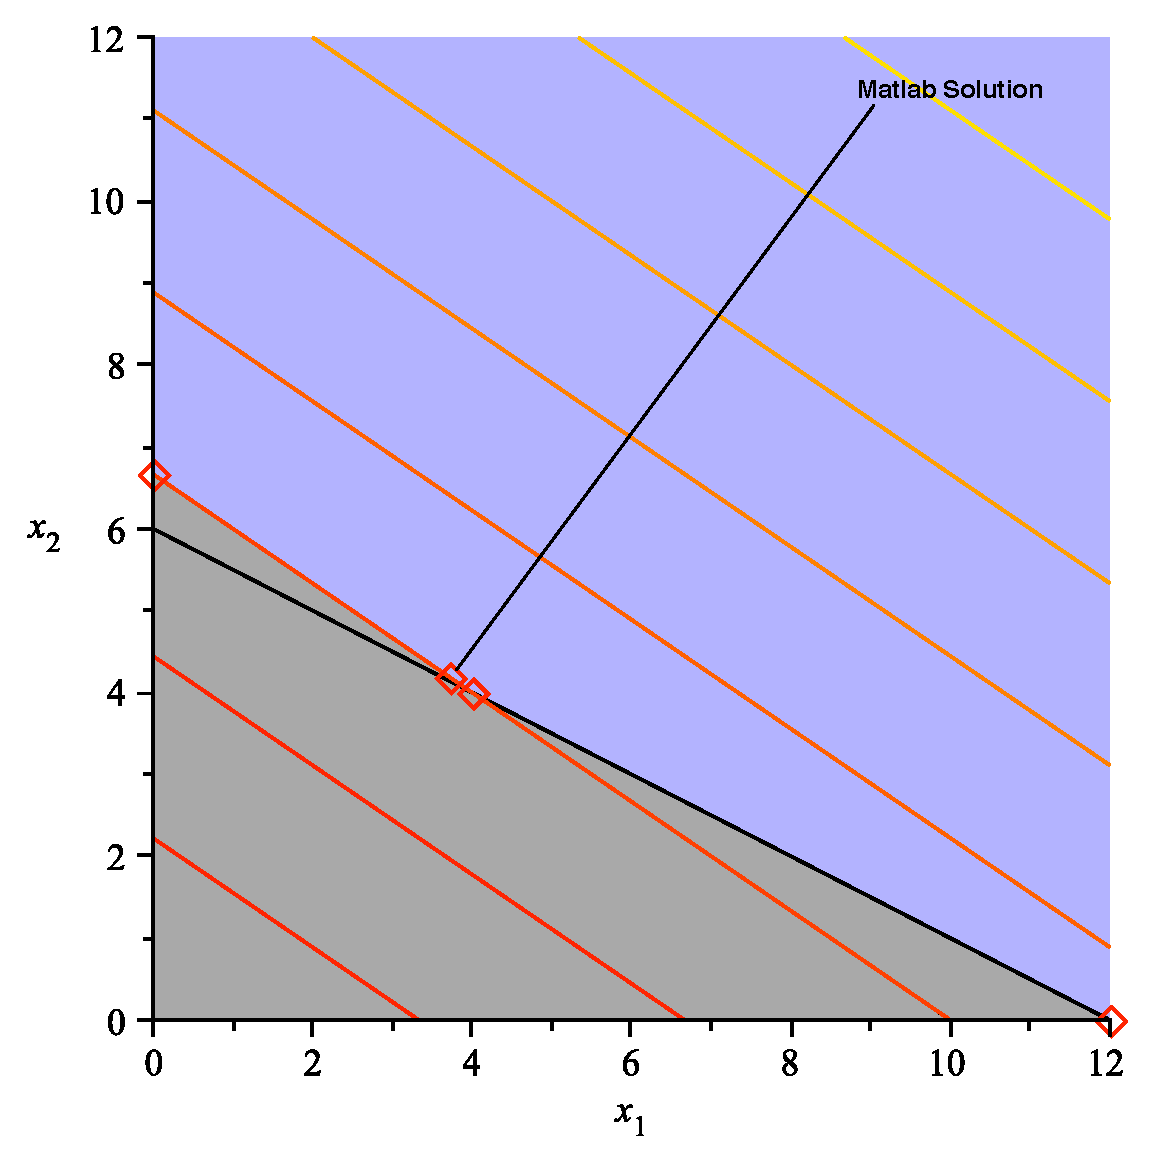
\includegraphics[scale=0.35]{DietProblemFigure.pdf}
\caption{The feasible region for the diet problem is unbounded and there are alternative optimal solutions, since we are seeking a minimum, we travel in the opposite direction of the gradient, so toward the origin to reduce the objective function value. Notice that the level curves hit one side of the boundary of the feasible region.}
\label{fig:DietProblem}
\end{figure}
If we continued in this way, we could actually construct all the points of intersection that make up the boundary of the feasible region. We'll can do one more, suppose $\mathbf{x}_\mathbf{B} = [x_1\;\;s_1]^T$. Then we would use Gauss-Jordan elimination to obtain:
\begin{displaymath}\left[
\begin{array}{cccc|c}
1 & 2 & 0 & -1 & 12\\
0 & 1 & 1 & -2 & 4
\end{array}\right]
\end{displaymath}
Notice there are now columns of the identity matrix in the columns corresponding to $s_1$ and $x_1$. That's how we know we're solving for $s_1$ and $x_2$. We have $x_1 = 12$ and $s_1 = 4$. By definition $x_1 = s_2 = 0$. This corresponds to the point $x_1 = 12, x_2 = 0$ shown in Figure \ref{fig:DietProblem}.

Let's use Matlab to solve this problem. Our original problem is:
\begin{displaymath}
\left\{
\begin{aligned}
\min\;\;& x_1 + 1.5x_2\\
s.t. \;\;& 2x_1 + 3x_2 \geq 20\\
& x_1 + 2x_2 \geq 12\\
&x_1, x_2 \geq 0
\end{aligned}\right.
\end{displaymath}

This is not in a form Matlab likes, so we change it by multiplying the constraints by $-1$ on both sides to obtain:
\begin{displaymath}
\left\{
\begin{aligned}
\min\;\;& x_1 + 1.5x_2\\
s.t. \;\;& -2x_1 - 3x_2 \leq -20\\
& -x_1 - 2x_2 \leq -12\\
&x_1, x_2 \geq 0
\end{aligned}\right.
\end{displaymath}

Then we have:
\begin{gather*}
\mathbf{c} = \begin{bmatrix}1\\1.5\end{bmatrix}\\
\mathbf{A} = \begin{bmatrix}-2 & -3\\-1 & -2\end{bmatrix}\\
\mathbf{b} = \begin{bmatrix}-20\\-12\end{bmatrix}\\
\mathbf{H} = \mathbf{r} = []\\
\mathbf{l} = \begin{bmatrix}0\\0\end{bmatrix}
\mathbf{u} = []
\end{gather*}
The Matlab code to solve this problem is shown in Figure \ref{fig:MatlabDiet}
\begin{figure}[htbp]
\centering
\scriptsize
\verbatiminput{SolveDietProblem.m}
\normalsize
\caption{Matlab input for solving the diet problem. Note that we are solving a \textit{minimization} problem. Matlab assumes all problems are \textit{mnimization} problems, so we don't need to multiply the objective by $-1$ like we would if we started with a maximization problem.}
\label{fig:MatlabDiet}
\end{figure}
The solution Matlab returns in the \texttt{x} variable is $x_1 = 3.7184$ and $x_2 = 4.1877$, note this is on the line of alternative optimal solutions, but it is not at either end of the line. I prefer to have a little less ice cream, so I'd rather have the alternative optimal solution $x_1 = x_2 = 4$.
\label{ex:Diet}
\end{example}

\begin{exercise} In previous example, you could also have just used the problem in standard form with the surplus variables and had $\mathbf{A} = \mathbf{b} = []$ and defined $\mathbf{H}$ and $\mathbf{r}$ instead. Use Matlab to solve the diet problem in \textit{standard form}. Compare your results to Example \ref{ex:Diet}
\end{exercise}